Observa los dos triángulos congruentes de la Figura \ref{fig:congruencia03}  para responder cada pregunta.

\begin{minipage}{0.5\textwidth}
    \begin{parts}
        \part El ángulo E es congruente al ángulo \fillin[H][1cm].
        \part $\overline{FG} \cong$  \fillin[$\overline{IJ}$][1cm].
        \part El ángulo J es congruente al ángulo \fillin[G][1cm].
    \end{parts}
\end{minipage}%
\begin{minipage}{0.5\textwidth}
    \begin{figure}[H]
        \centering
        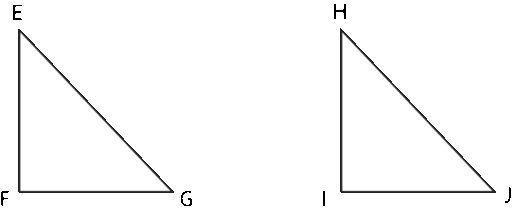
\includegraphics[width=\linewidth]{../images/congruencia03}
        \caption{}
        \label{fig:congruencia03}
    \end{figure}
\end{minipage}